\section{Quantization of Gauge Theories}

\lipsum[1]\TODO{Add introduction to the quantization of gauge theories.}

\subsection{Faddeev Popov Quantization}

The quantization of gauge theories necessitates special mathematical considerations to systematically construct a well-defined Quantum Field Theory (QFT) and its corresponding perturbative expansion. The fundamental problem becomes immediately clear within the path integral approach, where a naive path integral quantization yields a severely diverging result. Let us consider the illustrative case of the abelian \(U(1)\) theory, which describes free electromagnetism.

The classical action and the naive path integral are given by:
\begin{equation} \label{eq:naive_action_Z}
    \begin{aligned}
        S[A] & = \int d^4x \left( -\frac{1}{4}F_{\mu\nu}F^{\mu\nu} \right), \\
        Z    & = \int \mathcal{D}A \, e^{iS[A]} \to \infty,
    \end{aligned}
\end{equation}
where the electromagnetic field strength tensor is defined as \(F_{\mu\nu} = \partial_\mu A_\nu - \partial_\nu A_\mu\). Here, the path integral inherently diverges because one is redundantly summing over an infinite number of gauge-equivalent field configurations. Specifically, configurations related by the local gauge transformation
\begin{equation} \label{eq:gauge_transformation}
    A_\mu(x) \rightarrow A_\mu^g(x) = A_\mu(x) + i g(x)\partial_\mu g^{-1}(x) \, , \qquad g(x) = e^{i\alpha(x)} \in U(1),
\end{equation}
possess the exact same value of the action, \(S[A^g] = S[A]\). Consequently, the entire field space dynamically decomposes into inequivalent continuous \textbf{gauge orbits}, as visualized conceptually in the figure below.

\begin{figure}[H]
    \begin{minipage}{0.6\textwidth}
        \centering
        \definecolor{gaugeblue}{RGB}{20, 69, 120}
        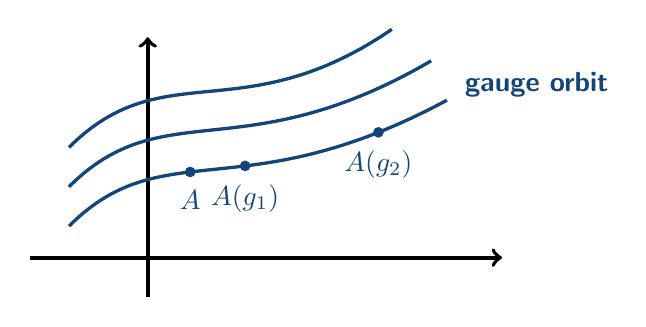
\begin{tikzpicture}[scale=1, thick, font=\sffamily]

            \draw[->, line width=1.4pt, rounded corners=1pt] (-1.5,0) -- (4.5,0);
            \draw[->, line width=1.4pt, rounded corners=1pt] (0,-0.5) -- (0,2.8);

            \draw[gaugeblue, line width=1.2pt] (-1, 0.4) .. controls (0.2, 1.6) and (1.2, 0.6) .. (3.8, 2.0)
            coordinate[pos=0.42] (pA)
            coordinate[pos=0.58] (pAg1)
            coordinate[pos=0.88] (pAg2);

            \draw[gaugeblue, line width=1.2pt] (-1, 0.9) .. controls (0.2, 2.1) and (1.2, 1.1) .. (3.6, 2.5);

            \draw[gaugeblue, line width=1.2pt] (-1, 1.4) .. controls (0.2, 2.6) and (1.2, 1.6) .. (3.1, 2.9);

            \filldraw[gaugeblue] (pA) circle (1.5pt) node[below=3pt] {$A$};
            \filldraw[gaugeblue] (pAg1) circle (1.5pt) node[below=3pt] {$A(g_1)$};
            \filldraw[gaugeblue] (pAg2) circle (1.5pt) node[below=3pt] {$A(g_2)$};

            \node[gaugeblue, right, font=\sffamily\bfseries] at (3.9, 2.2) {gauge orbit};

        \end{tikzpicture}
    \end{minipage}
    \hfill
    \begin{minipage}{0.35\textwidth}
        \caption{Gauge orbits in field space. The field configurations $A$, $A(g_1)$, and $A(g_2)$ lie on the same gauge orbit, meaning they are physically equivalent and connected by a gauge transformation $g(x) \in U(1)$.}
        \label{fig:gauge_orbits}
    \end{minipage}
\end{figure}

One would ideally like to formally define the path integral in such a way as to obtain a finite and explicitly gauge-invariant result by factoring out this redundant infinite volume:
\begin{equation} \label{eq:finite_path_integral}
    Z = \int \frac{\mathcal{D}A}{\text{Vol(Gauge)}} e^{iS[A]} \sim \text{finite},
\end{equation}
where the formal quantity ``Vol(Gauge)'' indicates the infinite volume of the gauge group. This conceptual definition can be implemented concretely using a \textit{gauge-fixing function \`a la Faddeev-Popov}, where unphysical ``ghost'' fields are elegantly introduced to exponentiate a crucial measure factor. Ideally, the chosen gauge-fixing function should pick exactly one single representative from each gauge orbit, as sketched in figure \ref{fig:gauge_fixing}. This idealized situation precisely corresponds to the choices of the so-called ``\textbf{unitary gauges}''. However, for practical perturbative calculations, it is often enough to merely reduce the number of representatives for each gauge orbit, which naturally happens in the standard choices of \textbf{covariant gauges}.

\begin{figure}[H]
    \begin{minipage}{0.35\textwidth}
        \caption{Gauge fixing by the condition $f(A) = 0$. The gauge-fixing function intersects the field space such that it picks ideally just one representative from each gauge orbit.}
        \label{fig:gauge_fixing}
    \end{minipage}
    \hfill
    \begin{minipage}{0.6\textwidth}
        \centering
        \definecolor{gaugeblue}{RGB}{20, 69, 120}
        \definecolor{gaugegreen}{RGB}{34, 139, 34}
        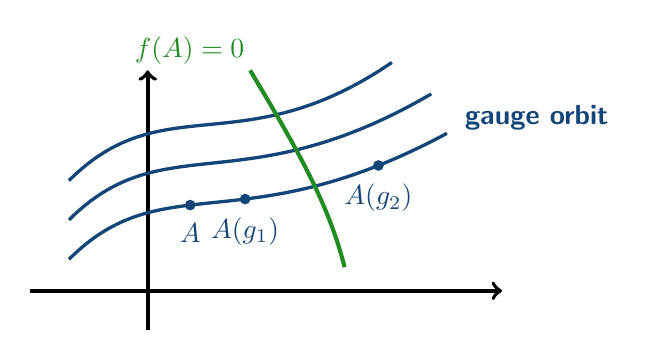
\begin{tikzpicture}[scale=1, thick, font=\sffamily]

            \draw[->, line width=1.4pt, rounded corners=1pt] (-1.5,0) -- (4.5,0);
            \draw[->, line width=1.4pt, rounded corners=1pt] (0,-0.5) -- (0,2.8);

            \draw[gaugeblue, line width=1.2pt] (-1, 0.4) .. controls (0.2, 1.6) and (1.2, 0.6) .. (3.8, 2.0)
            coordinate[pos=0.42] (pA)
            coordinate[pos=0.58] (pAg1)
            coordinate[pos=0.88] (pAg2);

            \draw[gaugeblue, line width=1.2pt] (-1, 0.9) .. controls (0.2, 2.1) and (1.2, 1.1) .. (3.6, 2.5);

            \draw[gaugeblue, line width=1.2pt] (-1, 1.4) .. controls (0.2, 2.6) and (1.2, 1.6) .. (3.1, 2.9);

            \draw[gaugegreen, line width=1.5pt] (1.3, 2.8) .. controls (1.9, 1.8) and (2.3, 1.1) .. (2.5, 0.3)
            node[pos=0, above left=-2pt, font=\sffamily\bfseries] {$f(A)=0$};

            \filldraw[gaugeblue] (pA) circle (1.5pt) node[below=3pt] {$A$};
            \filldraw[gaugeblue] (pAg1) circle (1.5pt) node[below=3pt] {$A(g_1)$};
            \filldraw[gaugeblue] (pAg2) circle (1.5pt) node[below=3pt] {$A(g_2)$};

            \node[gaugeblue, right, font=\sffamily\bfseries] at (3.9, 2.2) {gauge orbit};

        \end{tikzpicture}
    \end{minipage}
\end{figure}

As we shall explore, the gauge-fixed action thus obtained using covariant gauges exhibits a powerful residual global symmetry, called BRST symmetry. This symmetry is a direct remnant of the original gauge symmetry and is deeply instrumental in rigorously proving many properties of quantum gauge theories. In particular, it can be utilized to formally prove the independence of physical, observable quantities from the arbitrary choice of gauge-fixing function. It also forms the foundational basis of the BRST lagrangian quantization method, which systematically generalizes the Faddeev-Popov method to more complex, general cases. An even more powerful advanced method utilizes additional fields (the so-called antifields) and is widely known as the Batalin-Vilkovisky method.

\subsubsection{The Faddeev-Popov Trick}

Let us start by explicitly describing the Faddeev-Popov method in the simpler free abelian gauge theory case. The clever trick is to use a gauge-fixing condition, as depicted in figure \ref{fig:gauge_fixing}, and insert the identity (written in a suitable integral way) directly into the path integral to effectively extract the volume of the gauge group. Consider the elementary 1-dimensional identity written as:
\[1 = \int df \, \delta(f) = \int \frac{\partial f(y)}{\partial y} dy \, \delta(f(y)) = \int dy \, \delta(f(y)) \frac{\partial f(y)}{\partial y}\]
which smoothly generalizes to \(n\)-dimensions where \(f\) becomes a vector \(f^i\) with \(n\) components:
\[1 = \int d^n f \, \delta^{(n)}(f) = \int d^n y \, \delta^{(n)}(f(y)) \det \left( \frac{\partial f^i(y)}{\partial y^j} \right) \, .\]
We can formally generalize this finite-dimensional expression further to functional integrals over continuous fields:
\begin{equation} \label{eq:fp_identity}
    1 = \int \mathcal{D}g \, \delta\Big(f(A^g(x))\Big) \text{Det} \left( \frac{\delta f(A^g(x))}{\delta g(y)} \right)
\end{equation}
where \(\mathcal{D}g\) is a suitable gauge-invariant measure that also fundamentally produces the volume of the gauge group, \(\int \mathcal{D}g = \text{Vol(Gauge)}\). The notation ``Det'' strictly indicates a functional determinant. The delta function (which is actually a delta \textit{functional}) \(\delta(f(x))\) mathematically means that the whole function \(f(x)\) is strictly set to vanish.

Then, let us compute formally the path integral defined in \eqref{eq:finite_path_integral} by systematically inserting the functional identity from \eqref{eq:fp_identity}:
\[
    \begin{aligned}
        Z & = \int \frac{\mathcal{D}A}{\text{Vol(Gauge)}} e^{iS[A]} \\ &= \int \frac{\mathcal{D}A}{\text{Vol(Gauge)}} \int \mathcal{D}g \, \delta\Big(f(A^g(x))\Big) \text{Det} \left( \frac{\delta f(A^g(x))}{\delta g(y)} \right) e^{iS[A]} \\ &= \int \frac{\mathcal{D}A^g \mathcal{D}g}{\text{Vol(Gauge)}} \, \delta\Big(f(A^g(x))\Big) \text{Det} \left( \frac{\delta f(A^g(x))}{\delta g(y)} \right) e^{iS[A^g]} \\ &= \int \frac{\mathcal{D}g}{\text{Vol(Gauge)}} \int \mathcal{D}A \, \delta\Big(f(A(x))\Big) \text{Det} \left( \frac{\delta f(A^g(x))}{\delta g(y)} \right)\Bigg\vert{}_{g=1} e^{iS[A]} \\ &= \int \mathcal{D}A \, \delta\Big(f(A(x))\Big) \text{Det} \left( \frac{\delta f(A^g(x))}{\delta g(y)} \right)\Bigg\vert{}_{g=1} e^{iS[A]}
    \end{aligned}
\]
which is precisely the gauge-fixed path integral we were actively looking for. In these algebraic manipulations, we have first inserted the identity \eqref{eq:fp_identity}, and then utilized the fundamental fact that the action and the measure are both completely gauge invariant, namely \(S[A^g] = S[A]\) and \(\mathcal{D}A^g = \mathcal{D}A\). This is certainly mathematically true for the classical action, but it is an implicit assumption for the measure (more concretely, it is intimately related to the regularization methods used to make strict sense of the diverging Feynman diagrams characterizing the perturbative expansion\footnote{In chiral theories where the chosen regularization might fail to actively maintain gauge invariance, one physically speaks of \textbf{anomalies}. The entire quantization procedure breaks down if the potential anomalies in the gauge symmetry are not exactly canceled.}). Then, we have formally changed integration variables from \(A^g\) to \(A\), so that nothing in the integrand depends on the gauge parameter \(g(x)\) anymore. Consequently, the integration on \(\mathcal{D}g\) can be cleanly factorized out to exactly cancel the infinite gauge volume \(\text{Vol(Gauge)}\)\footnote{The formal mathematical identification \(\delta g \sim g^{-1} dg\) yields a strictly group-invariant measure, the so-called Haar measure.}.

The final formula is theoretically correct but can be elegantly written in a significantly more useful form by performing two essential steps:
\begin{itemize}
    \item[(i)] introducing \textbf{ghost fields}, i.e., anticommuting fields \(c(x)\) and \(\bar{c}(x)\) to exponentiate the functional determinant, broadly known as the Faddeev-Popov determinant,
    \item[(ii)] modifying the gauge-fixing function to effectively get rid of the rigid delta functional from the path integral: instead of strictly setting \(f(A(x)) = 0\), one may equivalently set it to \(f(A(x)) = h(x)\) (where \(h(x)\) is an arbitrary continuous function) and then functionally average over the diverse functions \(h(x)\) with a gaussian weight \(e^{-\frac{1}{2\xi} \int h^2}\).
\end{itemize}
The rigorous physical rationale behind this averaging procedure is that \uline{inherently different gauge- fixing functions must ultimately give the exact same gauge-invariant result}. In particular, nothing physical should depend on the specific numerical value of the gauge parameter \(\xi\).

Thus, implementing these exponentiation steps, one initially finds:
\[
    \begin{aligned}
        Z & = \int \mathcal{D}A \,\mathcal{D}c\, \mathcal{D}\bar{c}\, \mathcal{D}h \, \delta\Big(f(A(x)) - h(x)\Big)                                                           \\
          & \times \exp i \left( S[A] + \int d^4x d^4y \, \bar{c}(x) \frac{\delta f(A^g(x))}{\delta g(y)}\Bigg\vert{}_{g=1} c(y) - \frac{1}{2\xi} \int d^4x \, h^2(x) \right),
    \end{aligned}
\]
which is drastically simplified by path integrating over the auxiliary function \(h(x)\) to cleanly eliminate the delta functional, allowing us to find in the exponent the complete gauge-fixed total action \(S_{\text{tot}}\):
\begin{equation} \label{eq:path_integral_stot}
    \begin{aligned}
        Z & = \int \mathcal{D}A \mathcal{D}c \mathcal{D}\bar{c} \, \exp i \left( S[A] + \int d^4x d^4y \, \bar{c}(x) \frac{\delta f(A^g(x))}{\delta g(y)}\Bigg|_{g=1} c(y) - \frac{1}{2\xi} \int d^4x \, f^2(A(x)) \right) \\
          & = \int \mathcal{D}A \mathcal{D}c \mathcal{D}\bar{c} \, e^{i S_{\text{tot}}[A, c, \bar{c}]} \, ,
    \end{aligned}
\end{equation}
where the action appearing in the exponent has to be interpreted as the \textit{complete gauge-fixed action}.


\begin{example}[The Lorenz Gauge]
    To exemplify the abstract construction derived above, let us explicitly choose a specific gauge-fixing function:
    \begin{equation} \label{eq:lorenz_gauge_function}
        f(A) = \partial^\mu A_\mu,
    \end{equation}
    which corresponds directly to the strict \textit{Lorenz gauge} for the initial path integral derivation, and to a weighted Lorenz gauge for the path integral in \eqref{eq:path_integral_stot} (also frequently called the \(R_\xi\) gauge). Under an infinitesimal gauge variation \(\delta A_\mu = \partial_\mu \alpha\), the gauge-fixing function varies algebraically as:
    \[
        \delta f(A) = \partial^\mu \delta A_\mu = \partial^\mu \partial_\mu \alpha,
    \]
    and one is mathematically led to naturally interpret the functional derivative operator as:
    \[
        \frac{\delta f(A^g(x))}{\delta g(y)}\Bigg\vert{}_{g=1} \sim \frac{\delta f(A(x))}{\delta \alpha(y)} = \partial^\mu \partial_\mu \delta^4(x - y),
    \]
    whose functional determinant (the Faddeev-Popov determinant) can be faithfully reproduced by path integrating over the anti-commuting scalar ghost fields \(c(x)\) and \(\bar{c}(x)\). Thus, the complete gauge-fixed action reads:
    \begin{equation} \label{eq:stot_abelian}
        S_{\text{tot}}[A, c, \bar{c}] = S[A] + \int d^4x \left( -\partial^\mu \bar{c} \partial_\mu c - \frac{1}{2\xi} (\partial^\mu A_\mu)^2 \right) \, ,
    \end{equation}
    which is also called the \textit{quantum action} of the theory.

    The corresponding total gauge-fixed lagrangian density is given by:
    \begin{equation} \label{eq:ltot_abelian}
        \mathcal{L}_{\text{tot}} = -\frac{1}{4}F_{\mu\nu}F^{\mu\nu} - \partial^\mu \bar{c} \partial_\mu c - \frac{1}{2\xi}(\partial^\mu A_\mu)^2,
    \end{equation}
    which, up to total derivative terms that are usually dropped in the action since they do not affect equations of motion, may be symmetrically written as:
    \begin{equation} \label{eq:ltot_symmetric}
        \mathcal{L}_{\text{tot}} = -\frac{1}{2}\partial^\mu A^\nu \partial_\mu A_\nu + \frac{1}{2}\left(1 - \frac{1}{\xi}\right)(\partial^\mu A_\mu)^2 - \partial^\mu \bar{c} \partial_\mu c \, .
    \end{equation}
    In particular, the highly convenient Feynman gauge is obtained by setting \(\xi = 1\) and yields the remarkably simple action:
    \begin{equation} \label{eq:ltot_feynman}
        \mathcal{L}_{\text{tot}} = -\frac{1}{2}\partial^\mu A^\nu \partial_\mu A_\nu - \partial^\mu \bar{c} \partial_\mu c \, .
    \end{equation}

    Because the path integral is now perfectly well-defined, one can safely add external sources and compute the fundamental propagators of the theory. In the Feynman gauge, they read in momentum space:
    \begin{equation} \label{eq:propagators_feynman}
        \begin{aligned}
            \langle A_\mu(x) A_\nu(y) \rangle & = \int \frac{d^4p}{(2\pi)^4} \, e^{ip(x-y)} \frac{-i\eta_{\mu\nu}}{p^2 - i\epsilon} \\
            \langle c(x) \bar{c}(y) \rangle   & = \int \frac{d^4p}{(2\pi)^4} \, e^{ip(x-y)} \frac{-i}{p^2 - i\epsilon} \, .
        \end{aligned}
    \end{equation}
\end{example}

\textit{Exercise:} Find the exact form of the propagators in a generic \(R_\xi\) gauge.

At this advanced stage, one can also add matter fermions to obtain the complete QED action and critically note that the ghost fields can be safely integrated out and completely eliminated from the abelian theory. This is fundamentally because they contribute at most to an overall constant normalization factor that completely disappears when evaluating physically normalized correlation functions. This will decidedly not be the case for non-abelian gauge theories (and also for QED formulated in curved spacetime), but before mathematically addressing the more complex non-abelian case, let us discover and rigorously study a rigid symmetry that is robustly present in the gauge-fixed action and which has far-reaching physical implications, the BRST symmetry.

\subsection{BRST Symmetry}

Once the gauge symmetry has been fixed, the resulting gauge-fixed action \(S_{tot}\) is no longer gauge invariant. This is a necessary consequence, as the gauge-fixing term is explicitly introduced to break this redundancy and define a nonsingular path integral. However, a remnant of the original gauge symmetry survives in the form of BRST (Becchi-Rouet-Stora-Tyutin) symmetry, which is a rigid, global symmetry that depends on a constant, anticommuting (Grassmann-valued) parameter \(\Lambda\).

Let us consider the total lagrangian in the Feynman gauge:
\begin{equation} \label{eq:lagrangian_feynman}
    \mathcal{L}_{tot} = -\frac{1}{2}\partial^\mu A^\nu \partial_\mu A_\nu - \partial^\mu \bar{c} \partial_\mu c
\end{equation}
Under the BRST symmetry, the fields transform according to the following rules:
\begin{equation} \label{eq:brst_transformations}
    \begin{cases}
        \delta_B A_\mu(x) = \Lambda \partial_\mu c(x) \\
        \delta_B c(x) = 0                             \\
        \delta_B \bar{c}(x) = \Lambda \partial^\mu A_\mu(x)
    \end{cases}
\end{equation}
These transformations ensure that the variation of the total lagrangian vanishes up to total derivatives, meaning \(\delta_B \mathcal{L}_{tot} = 0\). It is important to recall that the transformation parameter \(\Lambda\), as well as the ghost fields \(c(x)\) and \(\bar{c}(x)\), are all Grassmann-valued quantities, which means they mutually anticommute.

A crucial, defining property of this symmetry is that it is nilpotent. Specifically, it is a Lie symmetry featuring a Grassmann odd parameter that satisfies the commutator relation:
\begin{equation} \label{eq:brst_commutator}
    [\delta_B(\Lambda_1), \delta_B(\Lambda_2)] = 0
\end{equation}
where one evaluates the variation using two different values of the constant Grassmann parameter, \(\Lambda_1\) and \(\Lambda_2\).

The nilpotency property becomes much more evident if one defines the Slavnov operator \(s\) by formally factorizing out the constant parameter \(\Lambda\):
\begin{equation} \label{eq:slavnov_definition}
    \delta_B(\Lambda) = \Lambda s \, .
\end{equation}
The Slavnov operator \(s\) acts as a nilpotent graded variation. In this context, "graded" indicates that the operator anticommutes with Grassmann odd fields, and "nilpotency" explicitly means that it satisfies the condition:
\begin{equation} \label{eq:slavnov_nilpotency}
    s^2 = 0
\end{equation}
Operating twice with \(s\) thus gives a vanishing result on any arbitrary field. Explicitly, extracting \(s\) from Eq. (\ref{eq:brst_transformations}), we get:
\begin{equation} \label{eq:slavnov_explicit}
    \begin{cases}
        s A_\mu(x) = \partial_\mu c(x) \\
        s c(x) = 0                     \\
        s \bar{c}(x) = \partial^\mu A_\mu(x)
    \end{cases}
\end{equation}
Applying the operator a second time confirms that it indeed gives zero:
\begin{equation} \label{eq:slavnov_squared}
    s^2 A_\mu(x) = s^2 c(x) = 0 \qquad \text{and} \qquad s^2 \bar{c}(x) = \partial^\mu \partial_\mu c(x) = 0
\end{equation}
Notice carefully that the classical ghost equations of motion (\(\partial^\mu \partial_\mu c = 0\)) have been used in the last equation to ensure the result vanishes. Because one strictly needs to use the equations of motion to satisfy \(s^2=0\), these particular BRST symmetry rules are said to be nilpotent \textit{on-shell}.

As for any rigid continuous symmetry, Noether's theorem guarantees there is an associated conserved current \(J_B^\mu\). This current can be found as usual by applying the Noether trick, which involves artificially extending the global parameter to a local one, \(\Lambda \rightarrow \Lambda(x)\), in Eq. (\ref{eq:brst_transformations}) and computing the variation of the action:
\begin{equation} \label{eq:brst_current}
    \delta_B S_{tot} = \int d^4x \, (\partial_\mu \Lambda) J_B^\mu \, , \qquad J_B^\mu = -F^{\mu\nu}\partial_\nu c - \partial^\nu A_\nu \partial^\mu c
\end{equation}
The associated conserved BRST charge \(Q_B\) is simply the spatial integral of the zero-component of this current:
\begin{equation} \label{eq:brst_charge}
    Q_B = \int d^3x \, J_B^0 = \int d^3x \left( \partial_\nu A^\nu \dot{c} - F^{0i}\partial_i c \right) \, .
\end{equation}
Upon canonical quantization, this classical charge mathematically becomes a nilpotent quantum operator: \(Q_B \rightarrow \hat{Q}_B\), satisfying \(\hat{Q}_B^2 = 0\).

There is an elegant theoretical way of adding auxiliary fields to the lagrangian to make the BRST symmetry nilpotent \textit{off-shell} (i.e., without requiring the equations of motion). To see how this remarkable property emerges, let us consider a Fourier path integral representation\footnote{This functional representation directly extends the usual one-dimensional formula for the Dirac delta function \(\delta(x) = \int \frac{dk}{2\pi} e^{-ikx}\) to the infinite-dimensional functional case.} of the delta functional utilized during the gauge-fixing procedure:
\begin{equation} \label{eq:delta_functional_path_integral}
    \delta(f(x)) = \int \mathcal{D}B \, e^{-i \int d^4x \, B(x) f(x)} \, ,
\end{equation}
We then substitute this functional representation directly into the gauge-fixed path integral. Subsequently, we path-integrate over the arbitrary gauge-weighting function \(h\) by standard Gaussian integration. The relevant part of the measure manipulations is given by:
\begin{equation} \label{eq:path_integral_manipulations}
    \begin{aligned}
        \int \mathcal{D}h \, & \delta\Big(f(A(x)) - h(x)\Big) e^{-i \int d^4x \, \frac{1}{2\xi} h^2(x)}                                           \\
                             & = \int \mathcal{D}h \mathcal{D}B \, e^{-i \int d^4x \, \left( B(x)[f(A(x)) - h(x)] + \frac{1}{2\xi}h^2(x) \right)} \\
                             & = \int \mathcal{D}B \, e^{i \int d^4x \, \left( -B(x)f(A(x)) + \frac{\xi}{2}B^2(x) \right)} \, .
    \end{aligned}
\end{equation}
From these algebraic manipulations, one naturally finds a new total lagrangian describing the extended set of fields \((A_\mu, c, \bar{c}, B)\). Given that we have previously taken the covariant gauge-fixing function to be \(f(A) = \partial^\mu A_\mu\), the lagrangian takes the updated form:
\begin{equation} \label{eq:lagrangian_off_shell}
    \mathcal{L}_{tot} = -\frac{1}{4}F_{\mu\nu}F^{\mu\nu} - \partial^\mu \bar{c} \partial_\mu c - B \partial^\mu A_\mu + \frac{\xi}{2}B^2 \, .
\end{equation}

With the introduction of the auxiliary field, the BRST symmetry transformations now read:
\begin{equation} \label{eq:brst_transformations_off_shell}
    \begin{cases}
        \delta_B A_\mu = \Lambda \partial_\mu c \\
        \delta_B c = 0                          \\
        \delta_B \bar{c} = \Lambda B            \\
        \delta_B B = 0
    \end{cases}
\end{equation}
This expanded set of transformations is manifestly nilpotent off-shell. Let us systematically recall the quantum statistics of the fields involved: the fields \(A_\mu\) and \(B\) are commuting (bosonic), while the ghost fields \(c\) and \(\bar{c}\) are anticommuting (fermionic). The field \(c(x)\) is explicitly called the \textit{ghost} and conceptually corresponds to the local gauge parameter \(\alpha(x)\), which in a profound sense is turned into a full dynamical field, but endowed with the opposite Grassmann character (\(\alpha(x) \rightarrow \Lambda c(x)\)). The field \(\bar{c}\) is analogously called the \textit{antighost}, while the newly introduced field \(B\) is the \textit{auxiliary field} (also widely known in literature as the Nakanishi-Lautrup field).

Of course, since \(B\) does not contain any derivative kinetic terms, one can easily eliminate it by using its purely algebraic equations of motion:
\begin{equation} \label{eq:b_equation_of_motion}
    B = \frac{1}{\xi} \partial^\mu A_\mu
\end{equation}
Substituting this back into the action, or equivalently, path-integrating over the \(B\) field in the functional integral, exactly reproduces the original lagrangian given in Eq. (\ref{eq:lagrangian_feynman}) (up to the \(\xi\) dependence). This explicitly checks that the new lagrangian provides a physically equivalent description of the exact same theory. However, eliminating the auxiliary field means that the BRST transformations reduce back to:
\begin{equation} \label{eq:brst_transformations_reduced}
    \begin{cases}
        \delta_B A_\mu = \Lambda \partial_\mu c \\
        \delta_B c = 0                          \\
        \delta_B \bar{c} = \frac{1}{\xi} \partial^\mu A_\mu \Lambda
    \end{cases}
\end{equation}
where strict nilpotency is unfortunately achieved only on-shell once again.

\subsection{Non-Abelian Gauge Fields}

[...]

\section{BRST Quantization}

 [...]

\subsection{Cohomology}

[...]

\subsection{Application: Gauge-Fixing of Perturbative Quantum Gravity}

[...]

\subsection{Graviton Propagator in Flat Spacetime}

[...]